\documentclass{article}

\title{EE 371 Autumn 2016 - Lab 2}
\date{\today}
\author{William Li, Dawn Liang, Jun Park}

% general document formatting
\usepackage[margin=1in]{geometry}
\usepackage[document]{ragged2e}
\usepackage{times}

\usepackage{titlesec}
\titleformat{\section}{\Large\bfseries}{\thesection}{0.5em}{\uppercase}

% formatting for code & floats
\usepackage{listings}
\usepackage{color}
\usepackage{graphicx}
\usepackage{float}
\usepackage{wrapfig}

\definecolor{dkgreen}{rgb}{0,0.6,0}
\definecolor{gray}{rgb}{0.5,0.5,0.5}
\definecolor{mauve}{rgb}{0.58,0,0.82}

\lstset{frame=tb,
  language=Verilog,
  aboveskip=3mm,
  belowskip=3mm,
  showstringspaces=false,
  columns=flexible,
  basicstyle={\small\ttfamily},
  numbers=none,
  numberstyle=\tiny\color{gray},
  keywordstyle=\color{blue},
  commentstyle=\color{dkgreen},
  stringstyle=\color{mauve},
  breaklines=true,
  breakatwhitespace=true,
  tabsize=3
}

\begin{document}

% signature page command
\newcommand{\namesigdate}[2][5cm]{
  \begin{tabular}{@{}p{#1}@{}}
    #2 \\[2\normalbaselineskip] \hrule \\[0pt]
    {\small \textit{Signature}} \\[2\normalbaselineskip] \hrule \\[0pt]
    {\small \textit{Date}}
  \end{tabular}
}

\pagenumbering{gobble}
\maketitle
\newpage

\paragraph{} We certify that the work in this report is our own, and that any work that is not ours is cited.

\paragraph{} \noindent \namesigdate{William Li} \hfill \namesigdate{Dawn Liang} \hfill \namesigdate{Jun Park}
\newpage

\paragraph{Contributions}

\tableofcontents
\newpage

\pagenumbering{arabic}

\section{Abstract}


\section{Introduction}


\section{Discussion}
\subsection{Design}
\subsubsection{Design Specification}
\subsubsection{Design Procedure}
\subsubsection{System Description}
\subsubsection{Software Implementation}
\subsubsection{Hardware Implementation}

\subsection{Test}
\subsubsection{Test Plan}
\subsubsection{Test Specification}
\subsubsection{Test Cases}


\section{Results}
\subsection{Analysis of Errors}


\section{Summary \& Conclusion}


\section{Appendix}
  \subsection{Two-scanner system}
    \subsubsection{Verilog code}
      % counter.v
      \lstinputlisting[language=Verilog]{../verilog/counter.v}
      \lstinputlisting[language=Verilog]{../verilog/counter_testbench.v}

      % counterCtrl.v
      \lstinputlisting[language=Verilog]{../verilog/counterCtrl.v}
      \lstinputlisting[language=Verilog]{../verilog/counterCtrl_testbench.v}

      % scannerState.v
      \lstinputlisting[language=Verilog]{../verilog/scannerState.v}
      \lstinputlisting[language=Verilog]{../verilog/scannerState_testbench.v}

      % scanner.v
      \lstinputlisting[language=Verilog]{../verilog/scanner.v}
      \lstinputlisting[language=Verilog]{../verilog/scanner_testbench.v}

      % overall.v
      \lstinputlisting[language=Verilog]{../verilog/overall.v}
      \lstinputlisting[language=Verilog]{../verilog/overall_testbench.v}

    \subsubsection{iverilog \& gtkwave waveforms}
      % counter gtkwave
      \begin{figure}[H]
        \centering
        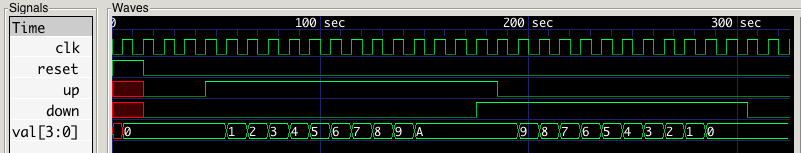
\includegraphics[width=0.75\linewidth]{figures/gtkwave/counter_gtkwave.png}
        \caption{counter module waveform}
        \label{fig:counter_gtkwave}
      \end{figure}

      % counterCtrl gtkwave
      \begin{figure}[H]
        \centering
        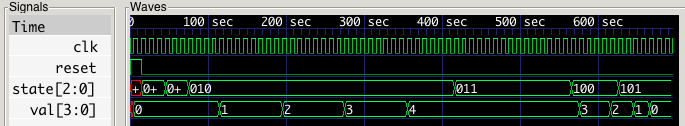
\includegraphics[width=0.75\linewidth]{figures/gtkwave/counterCtrl_gtkwave.png}
        \caption{counterCtrl module waveform}
        \label{fig:counterCtrl_gtkwave}
      \end{figure}

      % scannerState gtkwave
      \begin{figure}[H]
        \centering
        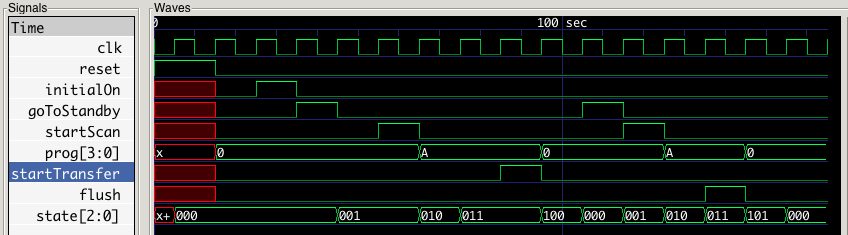
\includegraphics[width=0.75\linewidth]{figures/gtkwave/scannerState_gtkwave.png}
        \caption{scannerState module waveform}
        \label{fig:scannerState_gtkwave}
      \end{figure}

      % scanner gtkwave
      \begin{figure}[H]
        \centering
        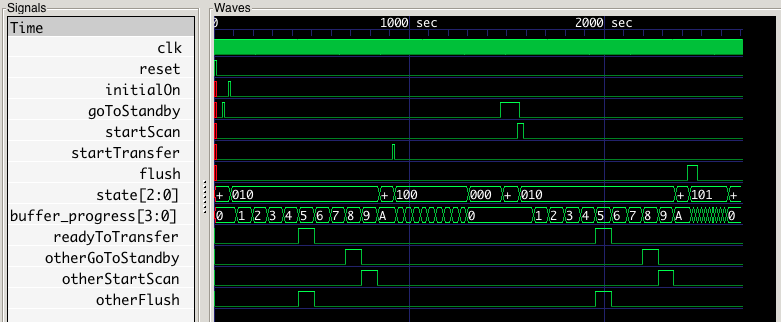
\includegraphics[width=0.75\linewidth]{figures/gtkwave/scanner_gtkwave.png}
        \caption{scanner module waveform}
        \label{fig:scanner_gtkwave}
      \end{figure}

      % overall gtkwave
      \begin{figure}[H]
        \centering
        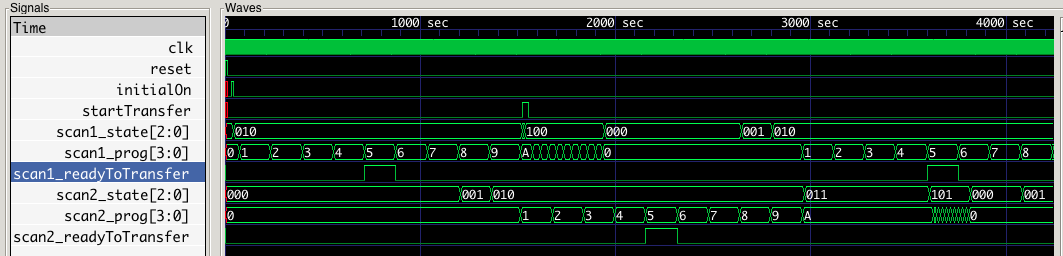
\includegraphics[width=0.75\linewidth]{figures/gtkwave/overall_gtkwave.png}
        \caption{overall module waveform}
        \label{fig:overall_gtkwave}
      \end{figure}

    \subsubsection{Signal Tap II data}

  \subsection{C Program}
    \lstinputlisting[language=C]{../c/calculateDelay.c}
    \lstinputlisting[language=C]{../c/temperature.c}

    % C program output
    \begin{figure}[H]
      \centering
      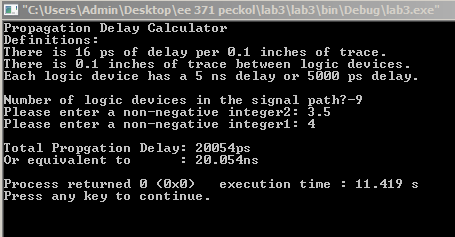
\includegraphics[width=0.75\linewidth]{figures/c/calculateDelay_output.png}
      \caption{Output of calculateDelay program}
      \label{fig:calculateDelay_output}
    \end{figure}

    \begin{figure}[H]
      \centering
      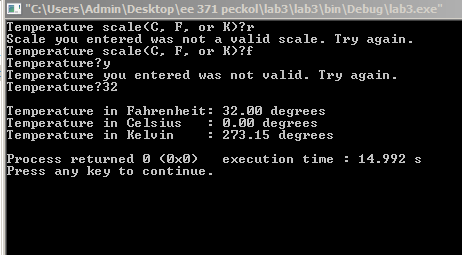
\includegraphics[width=0.75\linewidth]{figures/c/tempConv_output.png}
      \caption{Output of temperature program}
      \label{fig:tempConv_output}
    \end{figure}
\end{document}